\chapter{Asymptotic Normality of MLE}
\label{cha:Asymptotic Normality of MLE}

This chapter and the two chapters that follow develop asymptotic theory for likelihood-based statistical inference. Specifically, we will focus on maximum likelihood estimation (this chapter and Chapter 15) and likelihood ratio tests (Chapter 14).

For reading, consider Wellner (2018, chap. 4), Ferguson (1996, pt. 4), Lehmann
and Casella (1998, chap. 6).

%\section{Setup and a First Example}
%\label{setup-and-a-first-example}

\subsubsection{Setup}
\label{setup-3}

We consider the following standard statistical setup:
\begin{itemize}
	\item \textbf{Model:} We assume a parametric family of distributions:
	      \[ \mathcal{P} = \{ \mathsf{P}_{\boldsymbol{\theta}} \, : \, \boldsymbol{\theta} \in \Theta \}, \quad \Theta \subseteq \mathbb{R}^d. \]
	\item \textbf{Data:} We observe data points \(X_1, \dots, X_n\) which are independent and identically distributed (i.i.d.) according to the true distribution \(\mathsf{P}_{\boldsymbol{\theta}_0}\), where the true parameter \(\boldsymbol{\theta}_0\) lies in the interior of the parameter space \(\Theta\).
	\item \textbf{Likelihood:} We define the likelihood function \(L(\bs{\theta})\) and the log-likelihood function \(\ell(\bs{\theta})\) based on the densities \(p_{\bs{\theta}}\):
\end{itemize}

\[ L(\bs{\theta}) \equiv L_n(\bs{\theta}) = \prod_{i=1}^n p_{\bs{\theta}}(X_i), \]

\[ \ell(\bs{\theta}) \equiv \ell_n(\bs{\theta}) = \log L(\bs{\theta}) = \sum\limits_{i=1}^n \log p_{\bs{\theta}}(X_i). \]

The Maximum Likelihood Estimator (MLE), denoted as \(\hat{\bs{\theta}}_n\), is the parameter value that maximizes the probability of observing the data we actually saw.
\[ \hat{\bs{\theta}}_n = \arg\max_{\bs{\theta} \in \Theta} \ell_n(\bs{\theta}) \]
In sufficiently smooth models, this estimator solves the \textbf{likelihood equations}:
\[ \dot{\ell}(\boldsymbol{\theta}) \equiv \nabla_{\boldsymbol{\theta}} \, \ell(\boldsymbol{\theta}) = 0. \]

\paragraph{Intuition: The Link to KL Divergence}
Why do we maximize the likelihood? We can view the MLE as an estimator that attempts to minimize the Kullback-Leibler (KL) divergence between the empirical distribution of the data and the model distribution.
\[
\min_{\theta \in \Theta} KL(\widehat{\mathsf{P}}|\mathsf{P}_{\theta}) = \text{const.} - \max_{\theta \in \Theta} \frac{1}{n} \sum\limits_{i=1}^{n} \log p_{\theta}(X_i).
\]
In other words, finding the MLE is equivalent to finding the parameter \(\theta\) that makes the model distribution \(\mathsf{P}_\theta\) ``closest" (in the KL sense) to the observed data \(\widehat{\mathsf{P}}\).

\begin{note}[on Model Misspecification]
This perspective is particularly powerful because it explains what the MLE does even if our model is \textbf{wrong} (misspecified). If the true distribution \(\mathsf{P}\) is not in our model family \(\mathcal{P}\), the MLE will still converge to the parameter \(\theta^*\) that minimizes the KL divergence \(KL(\mathsf{P}|\mathsf{P}_{\theta})\). It finds the ``best approximating'' distribution within our (flawed) model class.
\end{note}

In the sequel, we consider an estimator \(\tilde{\theta}_n\) that is a \textbf{solution to the likelihood equations}, i.e., \(\dot{\ell}(\tilde{\theta}_n) = 0\), allowing for the case that \(\tilde{\theta}_n\) is merely a particular local maximum.

\begin{ex}[Gamma distribution model]
    
\label{example-13.1.-gamma-distribution-model}

Suppose \(X_1, ..., X_n\) are insurance claim sizes that we model as i.i.d. with a Gamma(\(\alpha, \beta\)) distribution, where \(\alpha > 0\) (shape) and \(\beta > 0\) (rate) are unknown. The density is given by:

\[ p_{\bs{\theta}}(x) = \frac{\beta^{\alpha}}{\Gamma(\alpha)} x^{\alpha - 1} e^{-\beta x} \cdot \mathbf{1}_{(0,\infty)}(x), \]

where \(\bs{\theta} = (\alpha, \beta)^{\top}\) and \(\Gamma(\alpha) = \int_0^{\infty} x^{\alpha - 1} e^{-x} dx\).

The log-likelihood function is:
\[ \ell(\bs{\theta}) = \sum\limits_{i=1}^{n} \left( \alpha \log(\beta) - \log \Gamma(\alpha) + (\alpha - 1) \log(X_i) - \beta X_i \right) \]
\[ = n\alpha \log(\beta) - n \log \Gamma(\alpha) + (\alpha - 1) \sum\limits_{i=1}^{n} \log(X_i) - \beta \sum\limits_{i=1}^{n} X_i. \]

The MLE depends on the sufficient statistics \(\sum\limits_{i=1}^{n} \log(X_i)\) and \(\sum\limits_{i=1}^{n} X_i\). However, taking derivatives and setting them to zero results in a system that cannot be solved ``in closed form'' for \(\alpha\) and \(\beta\).
This is a common situation in practice! Fortunately, it is no problem to compute the MLE via numerical optimization.
\end{ex}

\myparagraph{Illustration of consistency of MLE:}
We can define the negative log-likelihood function in R and minimize it using `optim'.

\begin{minted}{r}
negloglik <- function(ab, data){
    a <- ab[1]
    b <- ab[2]
    n <- length(data)
    return(
        -(n * a * log(b) - n * log(gamma(a))
        + (a - 1) * sum(log(data))
        - b * sum(data))
    )
}
\end{minted}

We simulate Gamma data with true parameters \(\alpha=5, \beta=2\):

\begin{minted}{r}
set.seed(22)
n <- 1000
x <- rgamma(n, shape = 5, rate = 2)
\end{minted}

We minimize the negative log-likelihood function based on \(n \in \{10, 100, 1000\}\) observations, starting with initial values \(\alpha = \beta = 1\).

\begin{minted}{r}
opt_10   <- optim(c(1, 1), negloglik, data = x[1:10])
opt_100  <- optim(c(1, 1), negloglik, data = x[1:100])
opt_1000 <- optim(c(1, 1), negloglik, data = x)
\end{minted}

The estimates for \(n = 10, 100\) and \(1000\) are:

\begin{minted}{r}
rbind(opt_10$par, opt_100$par, opt_1000$par)
#          [,1]     [,2]
# [1,] 9.755201 4.360160  <-- n=10 (Very noisy)
# [2,] 5.145909 1.954187  <-- n=100 (Better)
# [3,] 5.038665 2.031913  <-- n=1000 (Very close to truth 5, 2)
\end{minted}

\myparagraph{Illustration of asymptotic normality of MLE:}
To visualize the distribution of the estimator, we compute the MLE many times (10,000 simulations) for a fixed sample size \(n = 500\).

\begin{minted}{r}
set.seed(22)
Sims <- 10000
n <- 500
df <- data.frame(a = numeric(Sims), b = numeric(Sims))

for(s in 1:Sims){
    x = rgamma(n, shape = 5, rate = 2)
    opt = optim(c(5,2), negloglik, data = x)
    df$a[s] = opt$par[1]
    df$b[s] = opt$par[2]
}
\end{minted}

We then plot the distribution of the estimates of \(\alpha\) and \(\beta\). To illustrate \textbf{joint} asymptotic normality (not just marginals), we also consider a linear combination, e.g., \(2\alpha - \beta\).

\begin{minted}{r}
p1 <- ggplot(df, aes(x = a)) +
  geom_histogram(aes(y = after_stat(density)), colour = "white") +
  geom_function(fun = dnorm,
          args = list(mean = mean(df$b),
                  sd = sd(df$b)),
          colour = "red", linewidth = 1.5) +
  labs(x = expression(paste("MLE of ", beta)))

p3 <- ggplot(df, aes(x = 2 * a - b)) +
 geom_histogram(aes(y = after_stat(density)), colour = "white") +
 geom_function(fun = dnorm,
          args = list(mean = mean(2*df$a - df$b),
                  sd = sd(2*df$a - df$b)),
          colour = "red", linewidth = 1.5) +
 labs(x = expression(paste("MLE of ", 2*alpha - beta)))

p1 + p2 + p3 + plot_layout(ncol = 2, axis_titles = "collect")
\end{minted}

\begin{figure}[htpb]
    \centering
    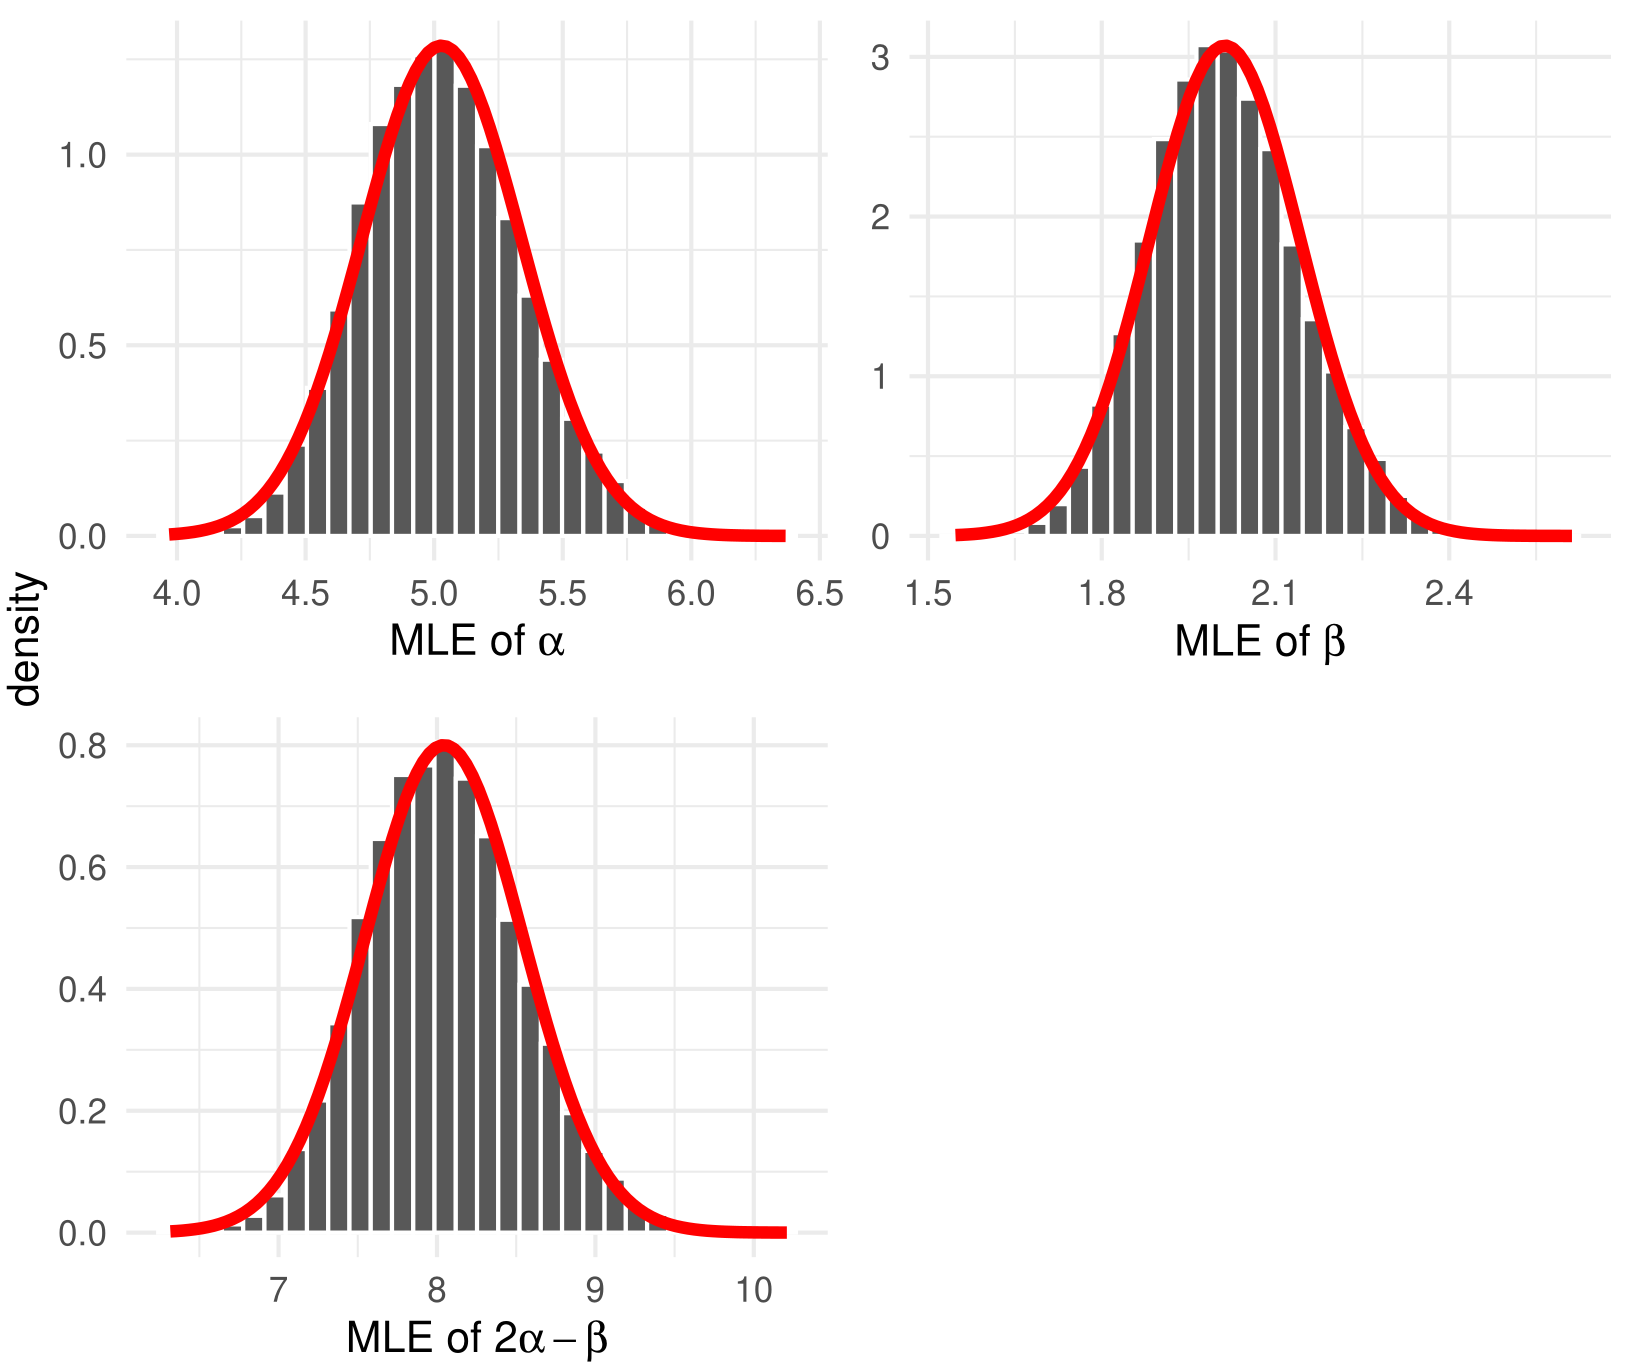
\includegraphics[width=0.8\textwidth]{./img/histograms}
    \caption{
Comparison between the empirical distribution (histogram) of the maximum likelihood
estimates for \(\alpha\), \(\beta\) and the linear combination \(2\alpha - \beta\), and a normal distribution (solid line)
with mean and variance being equal to the corresponding empirical moments.
    }
    \label{fig:histograms}
\end{figure}
The resulting histograms (\autoref{fig:histograms}) closely match the normal density curves (solid red lines), providing empirical evidence for the central limit theorem applied to MLEs.


\section{Consistency and Asymptotic Normality}
\label{sec:can}

\myparagraph{Assumptions for a general theorem}
To prove that the MLE behaves well (converges to the truth and is asymptotically normal), we need to ensure the log-likelihood function is sufficiently ``smooth" and well-behaved. We make the following assumptions:

\begin{enumerate}[label=\textbf{A\arabic*}, start=0]
    \item \textbf{(Identifiability):} \(\boldsymbol{\theta} \neq \boldsymbol{\theta}^* \implies \mathsf{P}_{\boldsymbol{\theta}} \neq \mathsf{P}_{\boldsymbol{\theta}^*}.\) Different parameters must correspond to different distributions; otherwise, we could never distinguish them based on data.
    \item \textbf{:} Densities \(p_{\theta}(x) = \frac{dP_{\theta}}{d\nu}(x)\) exist w.r.t. a \(\sigma\)-finite measure \(\nu\).
    \item \textbf{(Common Support):} \(A := \{x : p_{\bs{\theta}}(x) > 0\}\) does not depend on \(\bs{\theta}\). (This rules out cases like Uniform\((0, \bs{\theta})\), where the support boundary depends on the parameter, often breaking standard asymptotic theory).
    \item \textbf{(Smoothness):} On an open neighborhood \(\Theta_0\) of \(\bs{\theta}_0\), for \(\nu\)-a.e \(x\):
        \begin{enumerate}[label=\roman*)]
        \item \(\ell(\bs{\theta}|x) \equiv \log p_{\bs{\theta}}(x)\) is twice continuously differentiable in \(\bs{\theta}\).
        \item \(\ell(\bs{\theta}|x)\) has third-order derivatives 
        \[
            \dddot{\ell}_{jkl}(\bs{\theta}|x) = \frac{\partial ^3}{\partial \theta_{j} \partial \theta_{k}\partial\theta_{l}} 
            l(\bs{\theta}|x)
        \]
         bounded by an integrable function \(M(x)\):
        \[ |\dddot{\ell}_{ikl}(\boldsymbol{\bs{\theta}}|x)| \le M_{ikl}(x) \quad \forall \boldsymbol{\bs{\theta}} \in \bs{\theta}_0  \quad \forall 1\le j,k,l\le d,\]
        where \(\mathsf{E}_{\theta_0}\left[M_{jkl}(X_1)\right] <\infty \quad \forall j,k,l = 1,\dots ,d\).
    \end{enumerate}
    \textit{Intuition:} This control over the third derivative is crucial for the Taylor expansion argument. It ensures that the quadratic approximation of the log-likelihood dominates the higher-order terms (the ``wiggles'' of the function die out fast enough).
    \item \textbf{(Fisher Information):}
    \begin{enumerate}[label=\roman*)]
        \item The score function has mean zero: \(\mathsf{E}_{\boldsymbol{\bs{\theta}}_0}[\dot{\ell}_j(\boldsymbol{\bs{\theta}}_0|X_1)] = 0 \quad \forall j=1,\dots d\).
        \item The Fisher information \(\mathrm{I}(\bs{\theta}_0)=\mathsf{Var}_{\bs{\theta}_0}[\dot{\ell}(\bs{\theta}_0|X_1)]\) is finite.
        \item The Fisher information is positive definite and equals 
        \[
            I(\bs{\theta}_{0}) = \left(- \mathsf{E}_{\bs{\theta}_{0}}\left[\dddot{\ell}_{jk}(\bs{\theta}_{0}|X_1)\right] \right)_{jk}
        \]
        
    \end{enumerate}
\end{enumerate}

Our derivations will be driven by an application of the Central Limit Theorem (CLT) to the score function (gradient of the log-likelihood):
\[ \bs{Z}_n := \frac{1}{\sqrt{n}} \dot{\ell}(\boldsymbol{\theta}_0) = \frac{1}{\sqrt{n}} \sum\limits_{i=1}^n \dot{\ell}(\boldsymbol{\theta}_0 | X_i) \stackrel{d}{\longrightarrow} 
    \bs{Z}\sim \cc{N}_{d}\left( \bs{0},\mathsf{Var}_{\bs{\theta}_{0}}\left[\dot{l}(\bs{\theta}_{0}|X_1)\right]  \right) =
\bs{Z} \sim \mathcal{N}_d \big( \bs{0}, \bs{I}(\boldsymbol{\theta}_0) \big). \]

\begin{theo}[Consistency and Asymptotic Normality]
\label{theo:Consistency and Asymptotic Normality}
    
If assumptions A0-A4 hold, then:
\begin{enumerate}[label=\roman*.]
	\item \textbf{Consistency:} There exists a consistent sequence \(\tilde{\bs{\theta}}_n\) of solutions to the likelihood equations. That is,
	\[ \tilde{\bs{\theta}}_n \stackrel{p}{\longrightarrow} \bs{\theta}_0 \]
	and \(\mathsf{P}_{\bs{\theta}_0}(\tilde{\bs{\theta}}_n \text{ solves likelihood equations}) \longrightarrow 1\) as \(n \to \infty\).
	
\item 
    \label{ite:can2} 
    \textbf{Asymptotic Normality:} If \(\tilde{\bs{\theta}}_n\) satisfies the above, then
    \[ \sqrt{n}(\tilde{\bs{\theta}}_n - \bs{\theta}_0) = I(\bs{\theta}_0)^{-1} Z_n + o_p(1) \stackrel{d}{\longrightarrow} \mathcal{N}_d(\mathbf{0}, I(\bs{\theta}_0)^{-1}). \]
\end{enumerate}
\end{theo}

\begin{remark}[Clarification on Existence]
    The phrasing ``there exists a consistent sequence" can be technically subtle. It does not necessarily mean every root is consistent. However, for a concrete definition of \(\tilde{\bs{\theta}}_n\) used in proofs, one can define:
    \[
    \tilde{\bs{\theta}}_n = \begin{cases} 
    \text{solution closest to } \bs{\theta}_0, & \text{if } \exists \text{ solution to likelihood eqn's}, \\
    n \cdot \mathbf{1}, & \text{if } \nexists \text{ solution}.
    \end{cases}
    \]
    In practice, if the likelihood is unimodal (e.g., exponential families), the unique root is the MLE and is consistent. If the likelihood is multimodal, we typically select the root that maximizes the likelihood or is closest to a preliminary consistent estimator.
\end{remark}

    \begin{definition}[Asymptotically Linear Estimator]
    An estimator \(\hat{\bs{\gamma}}_n\) of parameter \(\bs{\gamma}\) is \textbf{asymptotically linear} if there exists a function \(h\) (called the \textbf{influence function}) such that:
    \[ \sqrt{n}(\hat{\bs{\gamma}}_n - \bs{\gamma}) = \frac{1}{\sqrt{n}} \sum_{i=1}^n h(X_i) + o_p(1). \]
    \end{definition}

\begin{remark}[on Influence Functions and Asymptotic Linearity]
    Part \ref{ite:can2} proves more than just normality; it proves the estimator is \textbf{asymptotically linear}.
    

    Our theorem shows that the consistent root \(\tilde{\bs{\theta}}_n\) is asymptotically linear with influence function:
    \[ h(X_i) = I(\bs{\theta}_0)^{-1} \dot{\ell}(\bs{\theta}_0 | X_i). \]
    
    \textbf{Why is this useful?}
    \begin{itemize}
        \item \textbf{Robustness:} The term ``influence function" comes from robust statistics. If \(h(X_i)\) is bounded, a single outlier cannot destroy the estimator (like the median). If \(h(X_i)\) is unbounded (like the mean), outliers can have a large effect.
        \item \textbf{Joint Distributions:} If we have two asymptotically linear estimators, say \(\hat{\bs{\gamma}}_n\) and \(\tilde{\bs{\theta}}_n\), we can easily derive their joint asymptotic distribution. By stacking their influence functions, the vector \((\hat{\bs{\gamma}}_n, \tilde{\bs{\theta}}_n)\) behaves like a sum of i.i.d. vectors, allowing us to apply the multivariate CLT to find asymptotic correlations.
    \end{itemize}
\end{remark}

TODO: detail this proof more
\begin{proof}[]
    \leavevmode
\begin{enumerate}
    \item \textbf{Existence and Consistency.}
    
    The proof relies on establishing that, with high probability, the log-likelihood function $\ell(\boldsymbol{\theta})$ has a local maximum within an arbitrarily small neighborhood of the true parameter $\boldsymbol{\theta}_0$.
    
    We define the boundary of a ball of radius $a$ centered at $\boldsymbol{\theta}_0$:
    \[ Q_a := \{\boldsymbol{\theta} \in \Theta : \|\boldsymbol{\theta} - \boldsymbol{\theta}_0\| = a\}. \]

    \begin{claim}[1]
    \label{claim:local_max}
    For any sufficiently small $a > 0$,
    \[ \mathsf{P}_{\boldsymbol{\theta}_0}(\ell(\boldsymbol{\theta}) < \ell(\boldsymbol{\theta}_0) \quad \forall \boldsymbol{\theta} \in Q_a) \longrightarrow 1 \quad \text{as } n \to \infty. \]
    \end{claim}
    
    If this claim holds, then with probability approaching 1, the continuous function $\ell(\boldsymbol{\theta})$ is strictly lower on the boundary $Q_a$ than at the center $\boldsymbol{\theta}_0$. Consequently, $\ell(\boldsymbol{\theta})$ must attain a local maximum at some point $\tilde{\boldsymbol{\theta}}_n$ in the interior of the ball (i.e., $\|\tilde{\boldsymbol{\theta}}_n - \boldsymbol{\theta}_0\| < a$). Since $\ell$ is differentiable, this local maximum satisfies the likelihood equations $\dot{\ell}(\tilde{\boldsymbol{\theta}}_n) = 0$.
    Since this holds for any $a > 0$, it implies the existence of a sequence of roots $\tilde{\boldsymbol{\theta}}_n$ such that $\tilde{\boldsymbol{\theta}}_n \stackrel{p}{\longrightarrow} \boldsymbol{\theta}_0$.

    \begin{proof}[of Claim \ref{claim:local_max}]
        
    %\textit{Proof of Claim \ref{claim:local_max}:}
    
    We perform a Taylor expansion of the log-likelihood around $\boldsymbol{\theta}_0$. Let $\boldsymbol{\theta} \in Q_a$.
    \[
    \frac{1}{n} [\ell(\boldsymbol{\theta}) - \ell(\boldsymbol{\theta}_0)] = S_{1n} + S_{2n} + R_n,
    \]
    where:
    \begin{itemize}
        \item \textbf{Linear term:} $S_{1n} = (\boldsymbol{\theta} - \boldsymbol{\theta}_0)^{\top} \left( \frac{1}{n} \dot{\ell}(\boldsymbol{\theta}_0) \right)$.
        \item \textbf{Quadratic term:} $S_{2n} = -\frac{1}{2} (\boldsymbol{\theta} - \boldsymbol{\theta}_0)^{\top} \left[ -\frac{1}{n} \ddot{\ell}(\boldsymbol{\theta}_0) \right] (\boldsymbol{\theta} - \boldsymbol{\theta}_0)$.
        \item \textbf{Remainder term:} $R_n$ involves third derivatives evaluated at some intermediate point $\boldsymbol{\theta}^*$ between $\boldsymbol{\theta}$ and $\boldsymbol{\theta}_0$.
    \end{itemize}

    We analyze the asymptotic behavior of each term as $n \to \infty$:

    \begin{enumerate}
        \item \textbf{Linear Term ($S_{1n}$):}
        By assumption A4, $\mathsf{E}[\dot{\ell}(\boldsymbol{\theta}_0)] = 0$. By the Law of Large Numbers (LLN), $\frac{1}{n} \dot{\ell}(\boldsymbol{\theta}_0) \stackrel{p}{\longrightarrow} 0$. Since $\|\boldsymbol{\theta} - \boldsymbol{\theta}_0\| = a$,
        \[ |S_{1n}| \le a \left\| \frac{1}{n} \dot{\ell}(\boldsymbol{\theta}_0) \right\| \stackrel{p}{\longrightarrow} 0. \]
        Thus, for any $\epsilon > 0$ (e.g., $a^3$), $|S_{1n}| < \frac{1}{2}a^3$ with high probability.

        \item \textbf{Quadratic Term ($S_{2n}$):}
        By the LLN, $-\frac{1}{n} \ddot{\ell}(\boldsymbol{\theta}_0) \stackrel{p}{\longrightarrow} I(\boldsymbol{\theta}_0)$.
        Since the Fisher Information matrix $I(\boldsymbol{\theta}_0)$ is positive definite, its smallest eigenvalue $\lambda_d > 0$.
        For sufficiently large $n$, the quadratic form behaves like:
        \[ S_{2n} \approx -\frac{1}{2} (\boldsymbol{\theta} - \boldsymbol{\theta}_0)^{\top} I(\boldsymbol{\theta}_0) (\boldsymbol{\theta} - \boldsymbol{\theta}_0). \]
        Using the eigenvalue bound:
        \[ (\boldsymbol{\theta} - \boldsymbol{\theta}_0)^{\top} I(\boldsymbol{\theta}_0) (\boldsymbol{\theta} - \boldsymbol{\theta}_0) \ge \lambda_d \|\boldsymbol{\theta} - \boldsymbol{\theta}_0\|^2 = \lambda_d a^2. \]
        Therefore, with high probability:
        \[ S_{2n} < -\frac{\lambda_d}{4} a^2 =: -C a^2 \quad (\text{where } C > 0). \]

        \item \textbf{Remainder Term ($R_n$):}
        Using the bound on third derivatives $M_{jkl}(x)$ from assumption A3:
        \[ |R_n| \le \frac{1}{6} \sum_{j,k,l} |\theta_j - \theta_{0j}| |\theta_k - \theta_{0k}| |\theta_l - \theta_{0l}| \left( \frac{1}{n} \sum_{i=1}^n M_{jkl}(X_i) \right). \]
        Since $\|\boldsymbol{\theta} - \boldsymbol{\theta}_0\| = a$, the product of differences scales with $a^3$. By the LLN, $\frac{1}{n} \sum M_{jkl}(X_i) \stackrel{p}{\longrightarrow} \mathsf{E}[M_{jkl}(X_1)]$.
        Thus, with high probability:
        \[ |R_n| \le B a^3 \quad (\text{where } B > 0 \text{ is a constant}). \]
    \end{enumerate}

    Combining these terms, on the sphere $Q_a$:
    \[ \frac{1}{n} [\ell(\boldsymbol{\theta}) - \ell(\boldsymbol{\theta}_0)] \le \frac{1}{2}a^3 - C a^2 + B a^3 = a^2 ( (B + 1/2)a - C ). \]
    For sufficiently small $a$ (specifically $a < \frac{C}{B + 1/2}$), the negative quadratic term $-C a^2$ dominates the cubic terms. Thus, the expression is strictly negative.
    
    This proves that $\ell(\boldsymbol{\theta}) < \ell(\boldsymbol{\theta}_0)$ for all $\boldsymbol{\theta} \in Q_a$ with probability approaching 1.
    \end{proof}

    \item \textbf{Asymptotic Normality.}
    
    Let $\tilde{\boldsymbol{\theta}}_n$ be the consistent sequence of roots found in part 1. We start by Taylor expanding the score function $\dot{\ell}(\tilde{\boldsymbol{\theta}}_n)$ around $\boldsymbol{\theta}_0$. Since $\tilde{\boldsymbol{\theta}}_n$ is a root, $\dot{\ell}(\tilde{\boldsymbol{\theta}}_n) = 0$.
    
    For the $j$-th component:
    \[
    0 = \dot{\ell}_j(\tilde{\boldsymbol{\theta}}_n) = \dot{\ell}_j(\boldsymbol{\theta}_0) + \left[ \nabla \dot{\ell}_j(\boldsymbol{\theta}_0) \right]^\top (\tilde{\boldsymbol{\theta}}_n - \boldsymbol{\theta}_0) + \frac{1}{2} (\tilde{\boldsymbol{\theta}}_n - \boldsymbol{\theta}_0)^\top \nabla^2 \dot{\ell}_j(\boldsymbol{\theta}_{n,j}^*) (\tilde{\boldsymbol{\theta}}_n - \boldsymbol{\theta}_0),
    \]
    where $\boldsymbol{\theta}_{n,j}^*$ lies between $\tilde{\boldsymbol{\theta}}_n$ and $\boldsymbol{\theta}_0$. Since $\tilde{\boldsymbol{\theta}}_n \stackrel{p}{\longrightarrow} \boldsymbol{\theta}_0$, we also have $\boldsymbol{\theta}_{n,j}^* \stackrel{p}{\longrightarrow} \boldsymbol{\theta}_0$.

    Rearranging terms to isolate the difference $(\tilde{\boldsymbol{\theta}}_n - \boldsymbol{\theta}_0)$:
    \[
    -\frac{1}{\sqrt{n}} \dot{\ell}_j(\boldsymbol{\theta}_0) = \left[ \frac{1}{n} \nabla \dot{\ell}_j(\boldsymbol{\theta}_0) + \text{Remainder}_j \right]^\top \sqrt{n}(\tilde{\boldsymbol{\theta}}_n - \boldsymbol{\theta}_0).
    \]
    
    We analyze the matrix in the brackets:
    \begin{itemize}
        \item The first term is the Hessian matrix of the log-likelihood (scaled by $1/n$). By the LLN:
        \[ \frac{1}{n} \nabla \dot{\ell}(\boldsymbol{\theta}_0) = \frac{1}{n} \ddot{\ell}(\boldsymbol{\theta}_0) \stackrel{p}{\longrightarrow} -I(\boldsymbol{\theta}_0). \]
        \item The remainder term involves third derivatives evaluated at $\boldsymbol{\theta}_{n,j}^*$. Using the bound $M_{jkl}(x)$ and the fact that $\|\tilde{\boldsymbol{\theta}}_n - \boldsymbol{\theta}_0\| \stackrel{p}{\longrightarrow} 0$, this term is $o_p(1)$.
    \end{itemize}

    Stacking all components $j=1,\dots,d$, we get the vector equation:
    \[
    -\frac{1}{\sqrt{n}} \dot{\ell}(\boldsymbol{\theta}_0) = \left[ -I(\boldsymbol{\theta}_0) + o_p(1) \right] \sqrt{n}(\tilde{\boldsymbol{\theta}}_n - \boldsymbol{\theta}_0).
    \]
    Multiplying by $-1$ and inverting the matrix (which converges to the invertible $I(\boldsymbol{\theta}_0)$):
    \[
    \sqrt{n}(\tilde{\boldsymbol{\theta}}_n - \boldsymbol{\theta}_0) = \left[ I(\boldsymbol{\theta}_0) + o_p(1) \right]^{-1} \frac{1}{\sqrt{n}} \dot{\ell}(\boldsymbol{\theta}_0).
    \]
    
    By the Central Limit Theorem, the normalized score function converges in distribution:
    \[ \mathbf{Z}_n = \frac{1}{\sqrt{n}} \dot{\ell}(\boldsymbol{\theta}_0) \xrightarrow{d} \mathcal{N}_d(\mathbf{0}, I(\boldsymbol{\theta}_0)). \]
    
    Using Slutsky's Theorem (\autoref{thm:slutsky}), we conclude:
    \[
    \sqrt{n}(\tilde{\boldsymbol{\theta}}_n - \boldsymbol{\theta}_0) \xrightarrow{d} I(\boldsymbol{\theta}_0)^{-1} \mathcal{N}_d(\mathbf{0}, I(\boldsymbol{\theta}_0)) = \mathcal{N}_d(\mathbf{0}, I(\boldsymbol{\theta}_0)^{-1}).
    \]
\end{enumerate}
\end{proof}

\section{One-Step Estimator}
\label{sec:One-Step Estimator}

In practice, the Maximum Likelihood Estimator (MLE) is often computed via iterative numerical optimization, typically using a Newton-type method. This requires an initialization and multiple iterations until convergence.

Interestingly, asymptotic theory suggests a remarkable shortcut: if we start with a ``decent'' preliminary estimator (one that is consistent and converges at a reasonable rate), performing just \textbf{one single Newton step} is sufficient to produce an estimator that shares the same asymptotic efficiency as the fully converged MLE.

\subsubsection{Optimization vs. Statistical Noise}
Why stop after one step? 

Optimization algorithms are designed to find the peak of the log-likelihood function $\ell_n(\theta)$ with high numerical precision. However, from a statistical perspective, the location of this peak (the MLE $\hat{\theta}_n$) is itself a random variable that fluctuates around the true parameter $\theta_0$ due to sampling noise. There is often little statistical gain in optimizing the likelihood function to a precision far beyond the inherent statistical noise of the problem. A one-step correction often brings the estimator within the range of statistical efficiency.

%\subsection{Definition and Theorem}
\bigskip

Let $\bar{\bs{\theta}}_n$ be a preliminary estimator. The one-step estimator $\check{\bs{\theta}}_n$ is defined by taking a single Newton step from $\bar{\bs{\theta}}_n$:

\begin{equation}
\label{eq:onestep_def}
\check{\bs{\theta}}_n := \bar{\bs{\theta}}_n + \hat{\mathbf{I}}(\bar{\bs{\theta}}_n)^{-1} \frac{1}{n} \dot{\ell}(\bar{\bs{\theta}}_n).
\end{equation}

Here, $\frac{1}{n} \dot{\ell}(\bar{\bs{\theta}}_n)$ is the gradient (score) scaled by sample size, and $\hat{\mathbf{I}}(\bar{\bs{\theta}}_n)$ is an estimator of the Fisher Information matrix. The Newton step essentially corrects the bias of the preliminary estimator using the curvature of the log-likelihood.

We can choose $\hat{\mathbf{I}}(\bs{\bs{\theta}})$ in several ways, all consistent for the true Fisher Information:

\begin{equation}
\hat{\mathbf{I}}(\bs{\theta}) = \begin{cases}
        \mathbf{I}(\bs{\theta}) & \text{(``Expected Fisher Information" -- Fisher Scoring)}, \\
        -\frac{1}{n} \sum\limits_{i=1}^{n} \ddot{\ell}(\bs{\theta}|X_i) & \text{(``Observed Fisher Information" -- Standard Newton)}, \\
        \frac{1}{n} \sum\limits_{i=1}^{n} \dot{\ell}(\bs{\theta}|X_i) \dot{\ell}(\bs{\theta}|X_i)^\top & \text{(Covariance of the Score)}.
\end{cases}
\end{equation}

\begin{remark}
    Using the observed Fisher information (the negative Hessian) corresponds to the standard Newton-Raphson method. Using the expected Fisher information is known as the \textbf{Fisher Scoring} algorithm. Asymptotically, these methods are equivalent because all three matrices converge to $\mathbf{I}(\theta_0)$.
\end{remark}

\begin{theo}[Asymptotic Normality of One-Step Estimator]
\label{theo:OneStep}
If assumptions A0-A4 hold and the preliminary estimator satisfies the condition
\[ n^{1/4}(\bar{\theta}_n - \theta_0) = o_p(1), \]
then the one-step estimator satisfies:
\[ \sqrt{n}(\check{\theta}_n-\theta_0) = \mathrm{I}(\theta_0)^{-1} \mathbf{Z}_n + o_p(1) \stackrel{d}{\longrightarrow} \mathcal{N}_d(\mathbf{0},\mathrm{I}(\theta_0)^{-1}). \]
\end{theo}

This theorem states that $\check{\theta}_n$ is asymptotically efficient (it achieves the Cramér-Rao lower bound), just like the MLE. The condition $n^{1/4}$ is weaker than the standard $\sqrt{n}$-consistency; essentially, the starting guess needs to be ``reasonably'' close to the truth, but not necessarily optimal.

\begin{proof}
    See, e.g., van der Vaart (1998, Theorem 5.45). The proof relies on Taylor expanding the score function and utilizing the consistency of the preliminary estimator.
\end{proof}

\medskip

\begin{ex}[Gamma Distribution]
    
\label{sub:Gamma_OneStep}

Consider the Gamma distribution model where $X_1, \ldots, X_n \sim \text{Gamma}(\alpha, \beta)$ are i.i.d. observations. The parameter vector is $\bs{\theta} = (\alpha, \beta)^{\top} \in \mathbb{R}^2_+$.

The Method of Moments (MoM) provides a convenient and consistent preliminary estimator $\overline{\bs{\theta}}$. By matching the first two theoretical moments ($E[X] = \alpha/\beta$, $Var(X) = \alpha/\beta^2$) with the sample moments, we obtain closed-form estimators:

\[
    \overline{\bs{\theta}} = \begin{pmatrix} \bar{\alpha}_n \\ \bar{\beta}_n \end{pmatrix} = \begin{pmatrix} \dfrac{\overline{X}_n^2}{\overline{X^2}_n - \overline{X}_n^2}, & \dfrac{\overline{X}_n}{\overline{X^2}_n - \overline{X}_n^2} \end{pmatrix}^{T}.
\]

These estimators are $\sqrt{n}$-consistent (and thus satisfy the $n^{1/4}$ requirement), but they are not efficient compared to the MLE. We can improve them using the one-step method.

\subsubsection{R implementation using `OneStep' package}
We simulate a dataset of size $n=1000$ from a Gamma(5, 2) distribution and compare the MoM estimator with the one-step improved version.

\begin{minted}[frame=lines, framesep=2mm, baselinestretch=1.2, fontsize=\footnotesize, linenos]{r}
library(OneStep)
n <- 1000
set.seed(1234)

# True parameters
theta_true <- c(5, 2)
# Generate data
x <- rgamma(n, shape = theta_true[1], rate = theta_true[2])

# 1. Compute Method of Moments (Preliminary Estimator)
# Note: mean(x^2) - mean(x)^2 is the biased sample variance
alpha_bar <- mean(x)^2 / (mean(x^2) - mean(x)^2)
beta_bar <- mean(x) / (mean(x^2) - mean(x)^2)

theta_bar <- list(shape = alpha_bar, rate = beta_bar)
print(theta_bar)
# $shape
# [1] 4.925981
# $rate
# [1] 1.950755
\end{minted}

The MoM estimates ($\approx 4.93, 1.95$) are decent but slightly off from the truth ($5, 2$). Now we apply the one-step correction:

\begin{minted}[frame=lines, framesep=2mm, baselinestretch=1.2, fontsize=\footnotesize, linenos]{r}
# 2. Apply One-Step Correction
onestep(x, "gamma", init = theta_bar)
# Parameters:
#        estimate Std. Error
# shape  5.082690         NA
# rate   2.012814         NA
\end{minted}

The improved estimate for $\beta$ ($\approx 2.01$) is closer to the true value of 2. Interestingly, if we run `onestep' without providing an initial value, it often defaults to using the Method of Moments internally:

\begin{minted}[frame=lines, framesep=2mm, baselinestretch=1.2, fontsize=\footnotesize, linenos]{r}
onestep(x, "gamma")
# Parameters:
#        estimate Std. Error
# shape  5.082690         NA
# rate   2.012814         NA
\end{minted}
\end{ex}

\section{Asymptotic Confidence Intervals}
\label{sec:Asymptotic Confidence Intervals}

We have derived the asymptotic normality of the MLE primarily to perform formal uncertainty assessments. Specifically, we want to construct confidence intervals for the true parameter $\theta_0$.

\subsection{Using Asymptotic Normality as a Pivot}
\label{sub:Using Asymptotic Normality}

Consider a one-parameter model ($d=1$), so $\Theta \subseteq \mathbb{R}$. Suppose $\tilde{\theta}_n$ is an estimator (like the MLE) such that for all $\theta_0 \in \Theta$:
\[
\sqrt{n}(\tilde{\theta}_n - \theta_0) \xrightarrow{d} \mathcal{N}(0, I(\theta_0)^{-1}).
\]
By Slutsky's Theorem (\autoref{thm:slutsky}), we can standardize this convergence. If we multiply by the square root of the Fisher Information $I(\theta_0)^{1/2}$, we obtain a pivotal quantity in the asymptotic sense:

\begin{equation}
\label{eq:asymp_pivot}
\sqrt{n} I(\theta_0)^{1/2} (\tilde{\theta}_n - \theta_0) \xrightarrow{d} \mathcal{N}(0, 1).
\end{equation}

\paragraph{Constructing the Interval}
We treat the left-hand side of \eqref{eq:asymp_pivot} as a pivot. Let $z_{\alpha/2}$ be the $(1 - \alpha/2)$ quantile of the standard normal distribution (e.g., 1.96 for $\alpha=0.05$). We define the confidence set $S_{\alpha}$ as the collection of all parameter values $\theta$ for which the pivot falls within the standard normal quantiles:

\begin{equation}
\label{eq:conf_set_def}
S_{\alpha} = \left\{ \theta \in \Theta : \left| \sqrt{n} I(\theta)^{1/2} (\tilde{\theta}_n - \theta) \right| \le z_{\alpha/2} \right\}.
\end{equation}

By construction, the coverage probability of this set converges to the target level:
\[
\mathsf{P}_{\theta}(\theta \in S_{\alpha}) \underset{n \to \infty}{\longrightarrow} \mathsf{P}(|\mathcal{N}(0, 1)| \le z_{\alpha/2}) = 1 - \alpha \quad \forall \theta \in \Theta.
\]
Thus, $S_{\alpha}$ is an asymptotic $(1 - \alpha)$ confidence interval.

\begin{ex}[Wilson Interval for Binomial Proportions]
    If the model is Binomial and $\theta$ is the success probability, this approach yields the \textbf{Wilson interval}.
    In this case, the Fisher information $I(\theta)$ depends on $\theta$ in a non-linear way ($I(\theta) = \frac{1}{\theta(1-\theta)}$). Solving the inequality in \eqref{eq:conf_set_def} requires solving a quadratic equation in $\theta$.
    
    The Wilson interval has interesting properties compared to simpler intervals (like the Wald interval discussed next). For instance, even if you observe extreme data (e.g., 0 successes in $n$ trials), the Wilson interval provides a non-trivial, positive-length interval, reflecting the inherent uncertainty more accurately than degenerate intervals.
\end{ex}

\begin{note}
    While conceptually sound, solving the inequality \eqref{eq:conf_set_def} for $\theta$ can be analytically difficult because $\theta$ appears in both the linear term $(\tilde{\theta}_n - \theta)$ and the information term $I(\theta)^{1/2}$. In general, $S_\alpha$ is not guaranteed to be a single connected interval, though it often is in exponential families like the Binomial.
\end{note}

\subsection{Wald Intervals}
\label{sub:Wald Intervals}

A very tractable construction of confidence intervals, which is the default in most statistical software, results from estimating the Fisher information. By Slutsky's theorem, we can replace the true Fisher information $I(\theta_0)$ with a consistent estimator $\hat{\mathbf{I}}(\tilde{\theta}_n)$ (e.g., the observed Fisher information evaluated at the MLE).

We have:
\[
\sqrt{n}\,\hat{\mathbf{I}}(\tilde{\theta}_n)^{1/2}(\tilde{\theta}_n-\theta_0)\stackrel{d}{\longrightarrow} \mathcal{N}(0,1).
\]
Based on this, the \textbf{Wald interval} is an asymptotic $(1 - \alpha)$ confidence interval defined as:
\[
W_{\alpha} = \left\{ \theta : \left| \sqrt{n} \, \hat{\mathbf{I}}(\tilde{\theta}_n)^{1/2} (\tilde{\theta}_n - \theta) \right| \le z_{\alpha/2} \right\} = \left[ \tilde{\theta}_n \pm z_{\alpha/2} \cdot \frac{1}{\sqrt{n \hat{\mathbf{I}}(\tilde{\theta}_n)}} \right].
\]
This interval is symmetric around the estimator $\tilde{\theta}_n$.

\paragraph{Multivariate Case ($d \ge 2$)}
This approach generalizes easily to intervals for individual components of a higher-dimensional parameter vector $\bs{\theta} \in \mathbb{R}^d$. The asymptotic normality result
\[
\sqrt{n}(\tilde{\bs{\theta}}_n - \bs{\theta}_0) \stackrel{d}{\longrightarrow} \mathcal{N}_d(0, I(\bs{\theta}_0)^{-1})
\]
implies convergence of the marginal distributions. For the $j$-th component:
\[
\sqrt{n}(\tilde{\theta}_{nj}-\theta_{0j}) \overset{d}{\longrightarrow} \mathcal{N}\left(0,\left(\mathrm{I}(\boldsymbol{\theta}_{0})^{-1}\right)_{jj}\right).
\]
Thus, an interval for the $j$-th component of $\bs{\theta}$ is formed as:
\[
W_{\alpha, j} = \left[\tilde{\theta}_{nj} \pm z_{\alpha/2} \cdot \sqrt{\frac{(\hat{\mathbf{I}}(\tilde{\bs{\theta}}_n)^{-1})_{jj}}{n}}\right].
\]
Here, $(\hat{\mathbf{I}}(\tilde{\bs{\theta}}_n)^{-1})_{jj}$ is the $j$-th diagonal element of the \textit{inverse} of the estimated Fisher information matrix.

\medskip

\begin{ex}[Wald intervals for the Gamma model]
We simulate data from a Gamma distribution and compute Wald intervals for its parameters.

\textbf{1. Computing the Interval:}
First, we define the negative log-likelihood and simulate 150 observations from a Gamma(5, 2) distribution.

\begin{minted}{r}
# Define negative log-likelihood (without 1/n scaling)
negloglik <- function(theta, data) {
  alpha <- theta[1]
  beta <- theta[2]
  n <- length(data)
  -sum(dgamma(data, shape = alpha, rate = beta, log = TRUE))
}

set.seed(22)
n <- 150
x <- rgamma(n, shape = 5, rate = 2)
\end{minted}

We optimize the likelihood and extract the Hessian (observed Fisher information) at the optimum.
\begin{minted}{r}
# hessian=TRUE requests the matrix of second derivatives
opt <- optim(c(1,1), negloglik, data = x, hessian = TRUE)
hat.theta <- opt$par
\end{minted}

We calculate the standard errors. Note that `\verb|opt$hessian|` computes $-\sum \ddot{\ell}$, so we must scale by $1/n$ to get the observed Fisher information $\hat{\mathbf{I}}$, invert it, and then scale by $1/n$ again for the variance of the estimator. Or equivalently, invert the raw Hessian directly.
The standard error (SE) is the square root of the diagonal elements of the inverse Hessian.

\begin{minted}{r}
# Inverse of the observed Fisher information matrix for the full sample
# opt$hessian is roughly n * I(theta)
var_matrix <- solve(opt$hessian) 
se <- sqrt(diag(var_matrix))
\end{minted}

Using the 0.975 quantile of $\mathcal{N}(0,1)$, we construct the intervals:
\begin{minted}{r}
z975 <- qnorm(0.975)
cbind(mle = hat.theta,
      lower = hat.theta - z975 * se,
      upper = hat.theta + z975 * se)
#           mle    lower    upper
# [1,] 5.458209 4.258774 6.657645  (alpha)
# [2,] 2.140010 1.647429 2.632591  (beta)
\end{minted}

\textbf{2. Checking Coverage Probability:}
To verify the validity of this interval, we can simulate the process 1000 times and check how often the true parameter $\alpha=5$ falls within the calculated interval.

\begin{minted}{r}
wald_ci_alpha_coverage <- function(n = 150, alpha = 5, beta = 2, conf.level = 0.95){
    x <- rgamma(n, shape = alpha, rate = beta)
    opt <- optim(c(1,1), negloglik, data = x, hessian = TRUE)
    
    hat.theta <- opt$par
    # Standard error for alpha (1st parameter)
    se_alpha <- sqrt(solve(opt$hessian)[1,1])
    
    quant <- qnorm(1 - (1 - conf.level)/2)
    
    # Check if true alpha is in interval
    lower <- hat.theta[1] - quant * se_alpha
    upper <- hat.theta[1] + quant * se_alpha
    
    return(alpha >= lower && alpha <= upper)
}

set.seed(22)
mean(replicate(1000, wald_ci_alpha_coverage()))
# [1] 0.944
\end{minted}
The estimated coverage is 94.4\%, which is very close to the nominal 95\% level, confirming the asymptotic theory works well for moderate sample sizes ($n=150$) in this regular model.
\end{ex}

\subsection{Optimality of the MLE}
\label{sub:Optimality of the MLE}

The MLE achieves the Cramér-Rao bound in an asymptotic sense: Its asymptotic covariance matrix is the inverse Fisher information. An estimator with this property is referred to as being \textbf{asymptotically efficient}.

However, making a rigorous statement about the asymptotic optimality of the MLE proved to be surprisingly difficult. While Fisher conjectured this efficiency in the 1920s, formal proofs took decades to materialize. The issue was settled in the 1960s and 70s with the \textbf{Hájek-Le Cam convolution theorem}.

\begin{note}
The convolution theorem:
\begin{itemize}
    \item Was proven decades after Fisher's initial conjecture.
    \item Restricts attention to \textbf{regular estimators} to avoid pathological counterexamples (see below).
    \item For details, see van der Vaart (1998, Chap. 8).
\end{itemize}
\end{note}

\paragraph{Why all this complexity?}
The main hurdle was the existence of ``superefficient" estimators—estimators that seemingly outperform the MLE (have lower asymptotic variance) at specific points in the parameter space.

\medskip

\begin{ex}[Hodges' Superefficient Estimator]
Suppose $d = 1$. Let $\hat{\theta}_n$ be the standard MLE such that for all $\theta \in \Theta$:
\[
\sqrt{n}(\hat{\theta}_n - \theta) \xrightarrow{d} \mathcal{N}(0, I(\theta)^{-1}).
\]
Fix a specific value $\theta_0 \in \Theta$. Define the Hodges estimator $\hat{\theta}_n^H$ as:
\[
\hat{\theta}_n^H := \begin{cases} 
\hat{\theta}_n & \text{if } n^{1/4} | \hat{\theta}_n - \theta_0 | > 1, \\ 
\theta_0 & \text{if } n^{1/4} | \hat{\theta}_n - \theta_0 | \leq 1. 
\end{cases}
\]
Essentially, this estimator checks if the MLE is close to $\theta_0$. If it is very close (within a $n^{-1/4}$ window), it snaps the estimate exactly to $\theta_0$.

As shown in Ferguson (1996, Example 1 on p. 134), the asymptotic distribution is:
\[
\sqrt{n}(\hat{\theta}_n^H - \theta) \xrightarrow{d} \mathcal{N}(0, V(\theta)), 
\quad \text{where } V(\theta) = \begin{cases} 
I(\theta)^{-1} & \text{if } \theta \neq \theta_0, \\ 
0 & \text{if } \theta = \theta_0. 
\end{cases}
\]
At $\theta = \theta_0$, the asymptotic variance is 0, which is strictly better than the MLE's variance $I(\theta_0)^{-1}$. Everywhere else, it matches the MLE. Thus, $\hat{\theta}_n^H$ appears to be ``superefficient."

\textbf{Why is this considered an artifact?}
While asymptotically superior at a single point, the Hodges estimator has terrible finite-sample performance near $\theta_0$. The risk (expected squared error) becomes very large in the transition region where the estimator switches between regimes. This superefficiency is an artifact of pointwise asymptotic comparisons that fails to capture the local behavior of the estimator.
\end{ex}

\paragraph{Regular Estimators and the Convolution Theorem}
To exclude pathological cases like the Hodges estimator, the Hájek-Le Cam theorem restricts the class of competitors to \textbf{regular estimators}.

\begin{definition}[Regular Estimator]
An estimator $T_n$ is regular if its asymptotic distribution is insensitive to small local perturbations of the parameter. Specifically, for local alternatives of the form $\bs{\theta}_n = \bs{\theta}_0 + \mathbf{t}/\sqrt{n}$, we require that the limiting distribution of $\sqrt{n}(T_n - \bs{\theta}_n)$ does not depend on $\mathbf{t}$.
\end{definition}

Under our standard assumptions, the MLE $\tilde{\bs{\theta}}_n$ is a regular estimator with asymptotic distribution $\mathcal{N}(0, \mathbf{I}(\bs{\theta}_0)^{-1})$. The convolution theorem states that among all regular estimators, the MLE has the smallest asymptotic variance (in a matrix sense). Any other regular estimator will have an asymptotic distribution equal to the MLE's distribution \textit{convolved} with independent noise, necessarily increasing the variance.

\subsection{Kullback-Leibler Divergence}
\label{sub:Kullback-Leibler Divergence}

The MLE can also be thought of as a plug-in estimator in the context of finding a distribution in the model that is as close as possible to the true data-generating distribution. This leads us to the concept of Kullback-Leibler (KL) divergence.

\begin{remark}
    Thinking about minimization of KL divergence offers a perspective that is helpful, in particular, when the model under consideration is \textbf{misspecified} (i.e., does not contain the true data-generating distribution). For example, if we model counts as Poisson when they are actually Negative Binomial, what is the MLE estimating?
\end{remark}

\begin{definition}[Kullback-Leibler Divergence]
    Let $\mathsf{P}$ and $\mathsf{Q}$ be probability distributions on $(\mathcal{X}, \mathcal{A})$ with densities $p$ and $q$ w.r.t. a $\sigma$-finite measure $\nu$. The Kullback-Leibler divergence from $\mathsf{P}$ to $\mathsf{Q}$ is
    \begin{equation*}
        KL(\mathsf{P}|\mathsf{Q}) = \mathsf{E}_{\mathsf{P}}\left[\log\frac{p(X)}{q(X)}\right]. \label{eq:KL_def}
    \end{equation*}
    (It does not depend on the choice of $\nu$.)
\end{definition}

\begin{note}
    KL divergence is not a distance/metric (it is not even symmetric, i.e., $KL(\mathsf{P}|\mathsf{Q}) \neq KL(\mathsf{Q}|\mathsf{P})$).
\end{note}

\begin{lemma}
    KL divergence is well-defined (as an integral) and
    \[
    KL(\mathsf{P}|\mathsf{Q}) \begin{cases} \in [0,\infty] & \textit{always}, \\ = 0  \iff& \mathsf{P} = \mathsf{Q}. \end{cases}
    \]
\end{lemma}

TODO: expand proofs with \(x\).
\begin{proof}[Well-definedness]
    Recall that $\log(x) \le x - 1$ for all $x > 0$. The KL divergence is well-defined if the negative part of $\log \frac{p(X)}{q(X)}$ has finite expectation under $\mathsf{P}$. This holds because:
    \[\begin{split} 
    \mathsf{E}_{\mathsf{P}} \bigg[ \max \bigg\{ -\log \frac{p(X)}{q(X)}, 0 \bigg\} \bigg] &= \int_{\{p \le q\}} \bigg( \log \frac{q}{p} \bigg) p \, \mathrm{d}\nu \\ 
    &\leq \int_{\{p \le q\}} \bigg( \frac{q}{p} - 1 \bigg) p \, \mathrm{d}\nu \\ 
    &\leq \int_{\{p \le q\}} (q - p) \, \mathrm{d}\nu \leq \int q \, \mathrm{d}\nu = 1. 
    \end{split}\]
\end{proof}

\begin{proof}[Non-negativity]
    \[\begin{aligned} 
    \mathsf{E}_{\mathsf{P}}\bigg[\log\frac{p(X)}{q(X)}\bigg] &= -\mathsf{E}_{\mathsf{P}}\bigg[\log\frac{q(X)}{p(X)}\bigg] \geq -\mathsf{E}_{\mathsf{P}}\bigg[\frac{q(X)}{p(X)} - 1\bigg] \\ 
    &= -\int_{\{p > 0\}} q \, \mathrm{d}\nu + 1 \geq -1 + 1 = 0. 
    \end{aligned}\]
\end{proof}

\begin{note}[]
    For \(KL(\mathsf{P}|\mathsf{Q}) < \infty\) it is necessary (but not sufficient) that \(\mathsf{P}\ll \mathsf{Q}\), i.e., \(\mathsf{Q}(A) = 0 \implies \mathsf{P}(A) = 0\) for all \(A \in \cc{A}\).
\end{note}

\begin{ex}[]
    \begin{align*}
    &p(x) = \bs{1}_{(0,1)}(x),\\
    &q(x) \propto e^{-\nicefrac{1}{x}}\bs{1}_{(0,1)}(x).
    \end{align*}
    %\(p(x) = \bs{1}_{(0,1)}(x),\quad  q(x) \propto e^{-\nicefrac{1}{x}}\bs{1}_{(0,1)}(x)  \).
\end{ex}

TODO: this proof is way longer.
\begin{proof}[Minimizer]
    Clearly $\mathsf{P}=\mathsf{Q} \implies KL=0$. For the converse, if $KL(\mathsf{P}|\mathsf{Q}) = 0$, then the non-negativity proof implies $\mathsf{E}_{\mathsf{P}}[\frac{q(X)}{p(X)} - 1 - \log\frac{q(X)}{p(X)}] = 0$. Since $x - 1 - \log x \ge 0$ with equality if and only if $x=1$, we must have $q(X)/p(X) = 1$ a.s. $[\mathsf{P}]$, implying $\mathsf{P}=\mathsf{Q}$.
\end{proof}

\subsubsection{Back to Estimation}
\label{sub:Back to Estimation}

Suppose $X_1, \dots, X_n \stackrel{\text{i.i.d.}}{\sim} \mathsf{P}$ (the true data-generating distribution), and we model this with a family $\mathcal{P} = \{\mathsf{P}_{\theta} : \theta \in \Theta\}$.

Which $\mathsf{P}_{\theta}$ is closest to $\mathsf{P}$ in the KL sense?


\[\begin{aligned} 
\min_{\theta \in \Theta} KL(\mathsf{P}|\mathsf{P}_{\theta}) &= \min_{\theta \in \Theta} \mathsf{E}_{\mathsf{P}} \Big[ \log \frac{p(X)}{p_{\theta}(X)} \Big] \\ 
&= \mathsf{E}_{\mathsf{P}} [\log p(X)] + \min_{\theta \in \Theta} \{ -\mathsf{E}_{\mathsf{P}} [\log p_{\theta}(X)] \} \\ 
&= \mathrm{const.} - \max_{\theta \in \Theta} \mathsf{E}_{\mathsf{P}} [\log p_{\theta}(X)]. 
\end{aligned}\]

If we replace the true expectation $\mathsf{E}_{\mathsf{P}}$ with the empirical average (plug-in the empirical distribution $\widehat{\mathsf{P}}$), we get:
\[
\max_{\theta \in \Theta} \frac{1}{n} \sum_{i=1}^{n} \log p_{\theta}(X_i).
\]
This is exactly the log-likelihood function!

\begin{remark}[Interpretation under Misspecification]
    We can interpret the MLE $\hat{\theta}_{\text{MLE}}$ as the parameter that minimizes the KL divergence between the empirical distribution and the model family.
    
    If the model is \textbf{misspecified} (i.e., $\mathsf{P} \notin \mathcal{P}$), the MLE converges to the parameter $\theta^*$ that minimizes $KL(\mathsf{P}|\mathsf{P}_{\theta})$.
    
\end{remark}
    \begin{ex}[Linear Regression]
        Suppose we fit a linear model $Y = \beta_0 + \beta_1 X + \epsilon$, but the true relationship is non-linear (e.g., quadratic). The MLE for the slope $\beta_1$ estimates the slope of the \textbf{best linear approximation} to the true curve in the KL sense (which corresponds to the best $L^2$ approximation for Gaussian errors).
    \end{ex}
    
    This theory is further developed in the context of \textbf{sandwich estimation}, where the asymptotic variance of the MLE takes a different form (``sandwich variance") because the cancellation between the Fisher information and the Hessian of the log-likelihood no longer holds.
